\section{State proofs in Solana}
State proofs are a necessary component of any blockchain to prove the existence or non-existence of a state object in the system. More generally, state proofs operate as follows:

\begin{itemize}
    \item \textbf{State commitment}: A state commitment $C_t$ is a succinct representation of the entire state of the system at a given point in time. This is used to ensure that the state has not been tampered with and can be used to verify the integrity of the state later using proofs $\pi$ (described below). Typically the state commitment is generated during the block-building time and is included in the block header. This block header is then signed by the block-builder and a supermajority of the validators in the system, effectively grounding its authority as the "source of truth".
    \item \textbf{State proof}: A state proof is a cryptographic proof that allows a user to verify the existence or non-existence of a state object in the system. This is typically done by creating a proof $\pi$ for a given key or a set of keys in the state. This proof later is verifiable against the state root.
    \item \textbf{Proof verification}: State proof verification is the process of verifying the state proof using the state commitment.
\end{itemize}

\begin{wrapfigure}{r}{0.60\textwidth}
    \centering
    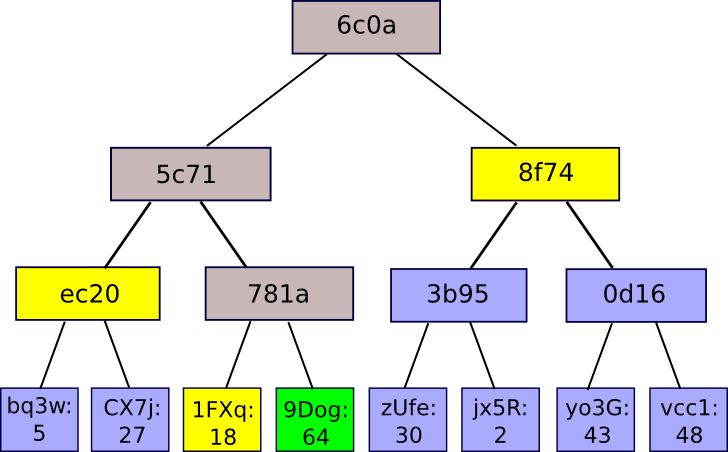
\includegraphics[width=0.60\textwidth]{solana/assets/merkle-proof-example.png}
    \caption{A example merkle proof: \textit{6c0a} is the state commitment, the topmost node of the binary merkle tree with 8 leaves. The proof for the key \textit{9Dog: 64} is the path from the leaf node to the root, hence \textit{[1FXq: 18, ec20, 8f74]} are additional data (state proof) against state commitment (6c0a) to prove existence of \textit{9Dog: 64}.}
    \label{fig:example-merkle-proof-solana}
\end{wrapfigure}

A classic example of state proofs is the Merkle tree. A Merkle tree is a binary tree where each leaf node is a hash of a data block and each non-leaf node is a hash of its children. The root of the tree is called the Merkle root and serves as the state commitment. The proof for a given key is the path from the leaf node to the root, which can be used to verify the existence or non-existence of the key in the state, see figure \ref{fig:example-merkle-proof-solana}.

\subsection{Homomorphic state commitment: \texttt{AccountsLatticeHash}}
Solana with two improvement documents: \href{https://github.com/solana-foundation/solana-improvement-documents/blob/main/proposals/0215-accounts-lattice-hash.md}{SIMD-0215} and \href{https://github.com/solana-foundation/solana-improvement-documents/blob/main/proposals/0223-removes-accounts-delta-hash.md}{SIMD-0223} proposes a new state commitment scheme called \textit{AccountsLatticeHash} and removal of previously existing \textit{AccountsDeltaHash} scheme.

More specifically, while SIMD-0215 proposes a new state commitment scheme (\texttt{AccountsLatticeHash}), SIMD-0223 proposes to remove the old scheme (\texttt{AccountsDeltaHash}).

Before introduction of the \texttt{AccountsLatticeHash}, solana used to have two main kinds of account hashes / state commitments:
\begin{itemize}
    \item The \textbf{Epoch Accounts Hash (EAH)}: This is a merkle tree hash of the full account data, sorted by public key, at the end of an "epoch" in solana.
    \item The \textbf{Accounts Delta Hash (ADH)}: This is a merkle tree hash of accounts, sorted by public key, written in a single block.
\end{itemize}

The epoch accounts hash is hash of a complete merkle tree and hence can by compared to a "full" state commitment, one against which a state proof for any key can be generated and verified. Ideally, this kind of "full" state commitment is what we want per block in any blockchain. However, generating this is quite expensive in terms of time and compute, leading to this requiring a time greater than 400ms, the average block generation time.

\subsubsection{The Lattice Hash Accumulator}
The Lattice Hash paradigm shifts from Merkle trees to a homomorphic hashing scheme. Each
account $a$ in the global state $S$ is assigned a unique cryptographic hash, denoted LtHash($D_a$),
where $D_a$ represents the account's complete data relevant for hashing (detailed below).

Each slot in the Solana blockchain has a unique \texttt{AccountsLatticeHash} represented by:
$$
\text{ALH} = \sum_{a \in S}{LtHash(D_a)}
$$
as such

Each account $a$ in the global state $S$ follows the following structure:
\begin{lstlisting}[language=Rust, caption=Account Structure in solana]
pub struct Account {
    pub account: Pubkey,    // 32 bytes, the key of the account in the state
    pub lamports: u64,      // 8 bytes, the number of lamports (tokens) in the account
    pub rent_epoch: Epoch,  // 8 bytes, the last epoch in which rent was paid for the account
    pub data: Vec<u8>,      // variable length, the data associated with the account, could be program, could be empty etc
    pub owner: Pubkey,      // 32 bytes, The public key of the program that owns the account
    pub executable: bool,   // 1 byte, whether the account is executable or not
}
\end{lstlisting}

\todo{Discuss about rent in solana}

Collectively, the metadata (excluding the variable "data") amounts to 81 bytes per account.
Thus, for an account with a 200-byte data field, the total input Da for its LtHash computation
would be 281 bytes.

The Solana blockchain typically sees around $10^2$ to $10^3$ accounts updates per slot. What this translates to in terms of \texttt{AccountsLatticeHash} is that the hash of the accounts in the next slot is computed as:

$$
\text{ALH}_{\text{new}} = \text{ALH}_{\text{old}} - \sum_{a \in S_m}{LtHash(D_{a, old})} + \sum_{a \in S_m}{LtHash(D_{a, new})}
$$

where $S_m$ is the set of accounts modified in the new slot. We assume $|S| \approx 10^3$ as of writing this document (22 May, 2025).

\subsection{Post-SIMD-223: \texttt{BankHash} composition}
Since SIMD 0223 remove the \texttt{AccountsDeltaHash} scheme, the \texttt{BankHash} now has:

\begin{lstlisting}[language=Rust, caption=Account Structure in solana]
pub struct BankHashComponents {
    pub parent_bank_hash: Hash,
    // pub accounts_delta_hash: Option<String>, // removed in SIMD-0223
    pub signature_count: u64,
    pub last_blockhash: Hash,
    pub epoch_accounts_hash: Option<String>,
    pub accounts_lt_hash_checksum: Option<String>,
    pub accounts: AccountsDetails,
}
pub struct BankHash {
    pub parent_hash: Hash,          // 32 bytes, the hash of the parent bank
    pub accounts_lt_hash: ALH,      // 2048-byte, the accounts lattice hash at given slot
    pub signature_count: u64,        // 8 bytes, the number of signatures in the bank
    pub last blockhash: Hash,      // 8 bytes, the number of transactions in the bank
}
\end{lstlisting}